\documentclass{article}

\usepackage[a4paper, total={6in, 8in}]{geometry}

\usepackage{amsmath}
\usepackage{amsfonts}
\usepackage{amssymb}
\usepackage[T1, T2A]{fontenc}
\usepackage[utf8]{inputenc}
\usepackage[english, russian]{babel}
\usepackage{graphics}
\usepackage{graphicx}
\usepackage{makecell}

\geometry{
 a4paper,
 total={170mm,257mm},
 left=20mm,
 top=20mm,
 }

\author{Александр Валентинов}
\title{Лабораторная работа 3.6.1}

\begin{document}
   \subsection*{Работа 3.3.4}
   \section*{Эффект Холла в полупроводниках}
   
   \paragraph{Цель работы:} измерение подвижности и концентрации носителей заряда в полупроводниках.
   
   \paragraph{В работе используются:} электромагнит с источником питания, амперметр, миллиамперметр, милливеберметр, реостат, цифровой вольтметр, источник питания ($1.5$В), образцы легированного германия.
   
   \subsubsection*{Экспериментальная установка:}
   
   \begin{figure}[h]
   \centering
   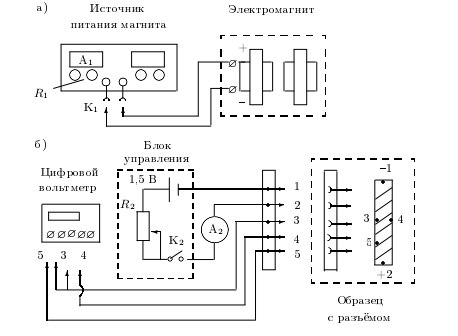
\includegraphics[width=8cm]{3_3_4.jpg} 
   \caption{Схема установки для исследования эффекта Холла в полупроводниках} 
   \label{fig.1} 
   \end{figure}

   \subsection*{Обработка результатов}
   Построим график зависимости $B(I_{\text{м}})$, чтобы определять индукцию магнитного поля по току в катушке (рис. \ref{fig.2}, табл. \ref{t1}). $\sigma_{I_{\text{м}}} = 0.01 \text{A}$, $\sigma_B$ пренебрежима мала.
   
   \begin{table}[h]
   \begin{center}
   \caption{Зависимость $B(I_{\text{м}})$}
   \label{t1}
   \begin{tabular}{|*{2}{r|}}
   \hline 
   $I_{\text{м}}$, А & $B$, мТл\\ \hline 
   0.00 & 17.2 \\ \hline 
   0.20 & 181.9 \\ \hline 
   0.40 & 378.1 \\ \hline 
   0.60 & 571.8 \\ \hline 
   0.80 & 730.7 \\ \hline 
   1.00 & 854.4 \\ \hline 
   1.20 & 934.9 \\ \hline 
   1.40 & 1,003.0 \\ \hline 
   \end{tabular}
   \end{center} 
   \end{table} 


   \begin{figure}[h]
   \centering
   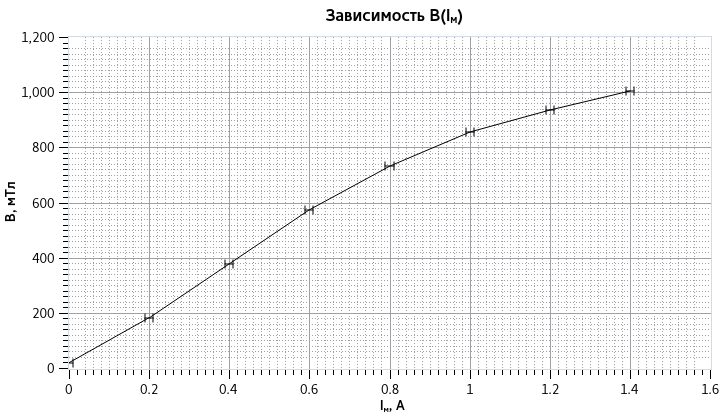
\includegraphics[width=15cm]{plot1.png} 
   \caption{Зависимость $B(I_{\text{м}})$} 
   \label{fig.2} 
   \end{figure}

   Рассчитаем ЭДС Холла по формуле 
   $$ \varepsilon_{\text{х}} = U_{34} - U_0 $$
   и построим графики  $\varepsilon_{\text{х}}(B)$ для различных $I_0$ (табл. \ref{exb1}, рис. \ref{fig.exb1}). Для каждого графика посчитаем коэффициент наклона $k(I_0) = \Delta\varepsilon / \Delta B$. Построим график $k = f(I_0)$ (табл. \ref{ki0}, рис. \ref{fig.ki0}). Коэффициент его наклона:
   $$ K = 87 \pm 8 \text{ В/(Тл$\cdot$А)} $$
   Выражение для коэффициента Холла:
   $$ \varepsilon_{\text{х}} = -R_{\text{х}} \cdot \frac{I_0B}{a},~~ \frac{\varepsilon_{\text{х}}}{B} = -\frac{R_{\text{х}}}{a} I_0,~~ k = KI_0,~~ K = \frac{R_\text{х}}{a}$$ 
   $$ R_{\text{х}} = -\frac{K}{a},~~ \sigma_{R_\text{х}} = \frac{K}{a^2}\sigma_a $$
   $$ R_\text{х} = (-0.087 \pm 0.004) ~~\text{м}^3 / \text{Кл} $$
   Концентрания носителей тока:
   $$ n = \frac{1}{R_xe},~~ \sigma_n = \frac{\sigma_{R_x}}{R_x^2e} $$
   $$ n = (7.0 \pm 0.3) \cdot 10^{19} ~ \text{м}^{-3} $$
   Результат совпадает с табличным значением $n \sim 10^{19}$ в пределах погрешности.

~

   \noindentРассчитаем удельную проводимость $\sigma$ по формуле:
   $$ \sigma = \frac{IL_{35}}{U_{35}al},~~ \sigma_{\sigma} = \frac{IL_{35}}{U_{35}al} \cdot \frac{\sigma_a}{a} $$
   $$ \sigma = (3.2 \pm 0.3)~ (\text{Ом$\cdot$м})^{-1} $$


   \noindentВычислим подвижность носителей тока:
   $$ b = \frac{\sigma}{en},~~ \sigma_b = \sqrt{\left(\frac{1}{en}\sigma_\sigma\right)^2 + \left(\frac{\sigma}{en^2}\sigma_n\right)^2} $$
   $$ b = (2900 \pm 300)~ \text{см}^2 / (\text{В} \cdot \text{с}) $$
   \begin{table}
   \begin{center}
   \caption{Зависимость $\varepsilon_{\text{х}}(B)$ для различных $I_0$}
   \label{exb1}
   \begin{tabular}{|*{8}{r|}}
   \hline 
   \multicolumn{1}{|c}{$I_0$, мА} & \multicolumn{1}{|c}{$0.30$} & \multicolumn{1}{|c}{$0.45$} & \multicolumn{1}{|c}{$0.50$} & 
   \multicolumn{1}{|c}{$0.65$} & \multicolumn{1}{|c}{$0.80$} & \multicolumn{1}{|c}{$0.95$} & \multicolumn{1}{|c|}{$0.95$ (обратно)} \\ \hline
   \multicolumn{1}{|c}{$B$, мТл} & \multicolumn{7}{|c|}{$\varepsilon_{\text{х}}$, мВ} \\ \hline 
   17.2 & 0.000 & 0.000 & 0.000 & 0.000 & 0.000 & 0.000 & 0.000 \\ \hline 
   181.9 & 0.051 & 0.072 & 0.084 & 0.109 & 0.129 & 0.159 & 0.166 \\ \hline 
   378.1 & 0.103 & 0.151 & 0.169 & 0.218 & 0.266 & 0.319 & 0.328 \\ \hline 
   571.8 & 0.151 & 0.224 & 0.251 & 0.322 & 0.396 & 0.472 & 0.496 \\ \hline 
   730.7 & 0.195 & 0.288 & 0.323 & 0.417 & 0.508 & 0.605 & 0.640 \\ \hline 
   854.4 & 0.228 & 0.336 & 0.378 & 0.487 & 0.595 & 0.710 & 0.750 \\ \hline 
   934.9 & 0.251 & 0.368 & 0.418 & 0.535 & 0.655 & 0.781 & 0.831 \\ \hline 
   1,003.0 & 0.269 & 0.394 & 0.446 & 0.569 & 0.698 & 0.830 & 0.884 \\ \hline 
   \end{tabular}
   \end{center} 
   \end{table} 

   \begin{figure}[h]
   \centering
   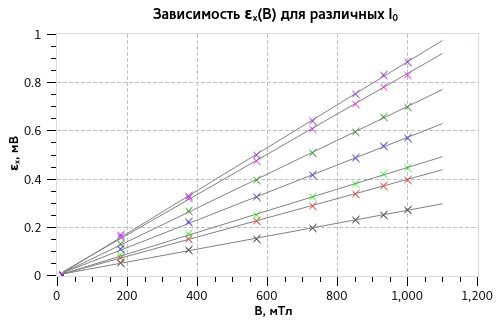
\includegraphics[width=12cm]{plot2.png} 
   \caption{Зависимость $\varepsilon_{\text{х}}(B)$ для различных $I_0$} 
   \label{fig.exb1} 
   \end{figure}

   \begin{table} 
   \begin{center}
   \caption{Зависимость $k(I_0)$}
   \label{ki0}
   \begin{tabular}{|*{3}{c|}}
   \hline 
   $I_0$, мА & $k$, мВ / мТл & $\sigma_k$, мВ / мТл \\ \hline 
   0.3 & 0.269 & 0.002 \\ \hline 
   0.45 & 0.397 & 0.003 \\ \hline 
   0.5 & 0.448 & 0.004 \\ \hline 
   0.65 & 0.573 & 0.005 \\ \hline 
   0.8 & 0.703 & 0.005 \\ \hline 
   0.95 & 0.835 & 0.008 \\ \hline 
   -0.95 & 0.891 & 0.007 \\ \hline 
   \end{tabular}
   \end{center}
   \end{table} 

   \begin{figure}[h]
   \centering
   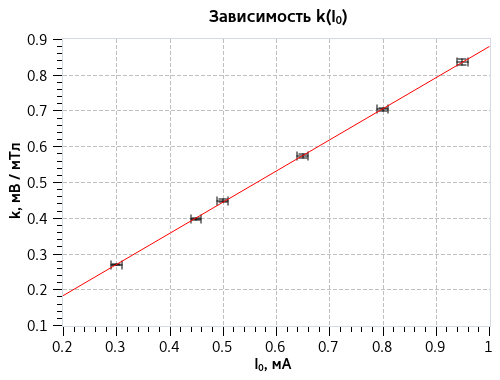
\includegraphics[width=12cm]{plot3.png} 
   \caption{Зависимость $k(I_0)$} 
   \label{fig.ki0} 
   \end{figure}

   \paragraph*{Вывод.} В ходе данной работы были получены значения постоянной Холла, удельной проводимости и подвижности носителей тока для германия.

\end{document}
